\begin{tcolorbox}[title={\Large グラフに対する教師付き学習}]
	\structure{入力}ラベル ($y$ : 離散, 実数値) 付きグラフ集合 \\
	\vspace{-85pt} \\
	\begin{center}
		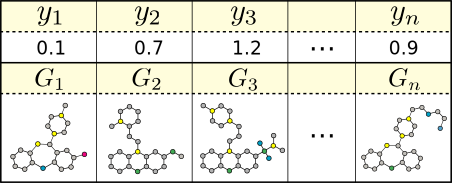
\includegraphics[width=470pt]{img/graph_classify.png}
	\end{center}
	\structure{出力}未知のグラフに対するラベルを予測する予測モデル \\
	\vspace{-25pt} \\
	\structure{特徴量}部分グラフ指示子 \\
	\vspace{-40pt}
	\begin{center}
		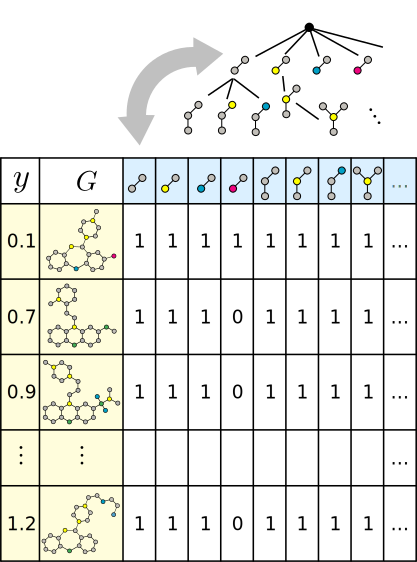
\includegraphics[width=470pt]{img/graph_indicator.png}
	\end{center}
	\vspace{-10pt}
	\structure{既存研究} 
	\begin{easylist}[itemize]
	@ 2-step 手法(Wale+ 2007) \\
	$~~~$ \alert{事前選択された特徴}の列挙 + 任意モデルでの学習 \\
	$~~~~~~~~ \rightarrow$ 事前に選択される特徴に大きく影響
	@ gBoost(Saigo+ 2009) \\
	$~~~$ 適応的部分グラフ指示子の探索・選択に基づく\alert{線形}モデル \\
	$~~~~~~~~ \rightarrow$ \express{全部分グラフ指示子}の考慮が可能
	\end{easylist}
\end{tcolorbox}

